\documentclass[11pt]{article}
\usepackage[margin=0.98in]{geometry}
\usepackage{amsmath,amssymb,booktabs}
\usepackage{graphicx}
\usepackage[expansion=false]{microtype}
\usepackage[font=small,labelfont=bf,skip=4pt]{caption}
\usepackage[colorlinks=true,linkcolor=black,citecolor=black,urlcolor=blue]{hyperref}
\usepackage{titlesec}
\titlespacing{\section}{0pt}{0.95em}{0.35em}
\titlespacing{\subsection}{0pt}{0.8em}{0.3em}
\setlength{\parskip}{0.22em}
\renewcommand{\topfraction}{0.92}
\renewcommand{\bottomfraction}{0.75}
\renewcommand{\textfraction}{0.06}
\renewcommand{\floatpagefraction}{0.85}
\newcommand{\rs}{$r^{*}$}
\begin{document}
\begin{center}
{\large\textbf{Disagreement in \boldmath$r^{*}$?}}\\[0.3em]
\end{center}
\vspace{0.1em}
\noindent\rule{\textwidth}{0.4pt}
\suppressfloats[t]
\vspace{0.2em}
% =====================================================================
\section{The question}
Long-term bond yields are anchored by beliefs about where short rates settle in the long run. A revision to that endpoint passes into the yield at every maturity, undamped by horizon, in a way that news about the current policy stance does not. This is why the endpoint has been at the center of the term-structure literature since Kozicki and Tinsley's shifting endpoints, and why Bauer and Rudebusch's falling stars put a slow-moving anchor at the heart of it. What is unsettled is where those beliefs come from, and whether the central bank is one of the sources.
Consider a policy rule written as follows,
\begin{equation}
i_t \;=\; \underbrace{r^{*}_t + \pi^{*}_t}_{\text{intercept}} \;+\; \phi_\pi\!\left(\pi_t - \pi^{*}_t\right) + \phi_x x_t + v_t ,
\label{eq:rule-general}
\end{equation}
\rs{} is the \emph{intercept} of the reaction function, so ``the Fed reveals \rs{}'' means the
Fed is telling markets about the constant in its own rule. Bauer, Pflueger \& Sunderam (2024)
estimate the perceived \emph{slope} $\phi_\pi$ and show it prices term premia; they absorb the
intercept into forecaster fixed effects. The intercept has been assumed
known, assumed common, or differenced away.
\begin{quote}
\textbf{How does the Fed move beliefs about the intercept of its own reaction function, and
what does disagreement about that intercept do to the price of long bonds?}
\end{quote}
\noindent In three parts:
\begin{enumerate}
    \item \textbf{Who moves whom}: Does the FOMC's published longer-run projection move primary dealers' beliefs about the same object, and by how much? And does the dealers' projection, which the Desk reports to the Committee before every meeting, move the FOMC's own, and by how much?
    \item \textbf{Pricing}: Does a revision to the published projection move the yield curve with the maturity profile of an endpoint shock? Can the term-premium response be separated from stance news and from a perceived policy error?
    \item \textbf{Disagreement}: Does dispersion in beliefs about the intercept carry a risk premium whose sensitivity does not decay with maturity? Does a signed Fed-minus-market gap move the level of yields, with the split between breakeven and real-rate responses pinned by the perceived rule?
\end{enumerate}
\clearpage
\section{Decomposing Long Yields}
Start from the definition of a long yield as an average of expected short rates plus a
residual:
\begin{equation}
y^{(n)}_t \;=\; \underbrace{\frac{1}{n}\sum_{j=0}^{n-1} E_t\!\left[i_{t+j}\right]}_{\text{expectations component } rn^{(n)}_t} \;+\; TP^{(n)}_t .
\label{eq:eh}
\end{equation}
Now split the nominal policy rate into a neutral level and a deviation from it. Define the
\emph{neutral nominal rate} and the \emph{policy gap}
\begin{equation}
i^{*}_t \;\equiv\; r^{*}_t + \pi^{*}_t ,
\qquad
\text{gap}_t \;\equiv\; i_t - i^{*}_t \;=\; \underbrace{\left(i_t - E_t\pi_{t+1} - r^{*}_t\right)}_{\text{real policy stance}} \;+\; \underbrace{\left(E_t\pi_{t+1} - \pi^{*}_t\right)}_{\text{inflation deviation}} ,
\label{eq:gapdef}
\end{equation}
where $r^{*}_t$ is the equilibrium real rate and $\pi^{*}_t$ the long-run inflation
anchor. The gap is therefore \textbf{the stance of policy}: how far the Fed is holding the
short rate above or below the level that would be neutral, plus how far inflation is
expected to run from its anchor. Under a Taylor-type rule
$i_t = i^{*}_t + \phi_\pi(\pi_t-\pi^{*}_t) + \phi_x x_t + v_t$, the gap is exactly the
systematic and discretionary response to the cycle,
\begin{equation}
\text{gap}_t \;=\; \phi_\pi\!\left(\pi_t-\pi^{*}_t\right) + \phi_x x_t + v_t .
\label{eq:taylor}
\end{equation}
Substituting \eqref{eq:gapdef} into \eqref{eq:eh}, and adding the martingale assumption for
the endpoints --- $E_t[r^{*}_{t+j}]=r^{*}_t$ and $E_t[\pi^{*}_{t+j}]=\pi^{*}_t$ --- gives
\begin{equation}
y^{(n)}_t \;=\; r^{*}_t \;+\; \pi^{*}_t \;+\; \frac{1}{n}\sum_{j=0}^{n-1} E_t\!\left[\text{gap}_{t+j}\right] \;+\; TP^{(n)}_t .
\label{eq:identity}
\end{equation}
Equivalently, in terms of the neutral nominal rate,
\begin{equation}
y^{(n)}_t \;=\; i^{*}_t \;+\; \frac{1}{n}\sum_{j=0}^{n-1} E_t\!\left[\text{gap}_{t+j}\right] \;+\; TP^{(n)}_t .
\label{eq:identity-istar}
\end{equation}
% From (4) we have that the gap at each time $t$ is equivelent to the Fed's policy response at that time. If the Fed's Policy Response is AR(1) with persistance $\rho$ we further decompose,
% Hillenbrand's evidence that the window decline is not the policy cycle is that it survives in the 5-year, 5-year-forward rate. That argument requires the expected stance to contribute negligibly at long horizons. It does not. The expected-gap term in \eqref{eq:identity} enters the ten-year yield with a weight of roughly 0.5 — estimated from the stance's own dynamics and stable between 0.51 and 0.55 across every specification I fit — so a 100 bp revision to the expected stance moves the ten-year about 50 bp and the 5y5y forward about 30 bp. The far-forward evidence does not separate endpoint news from stance news.
% and over an announcement window,
% \begin{equation}
% \Delta y^{(n)}_t \;=\; \underbrace{\Delta i^{*}_t}_{\text{endpoint news}}
% \;+\; \underbrace{\omega\,\Delta\text{gap}_t + \text{gap}_t\,\Delta\omega}_{\text{stance and persistence news}}
% \;+\; \Delta TP^{(n)}_t .
% \label{eq:windowdiff}
% \end{equation}
\clearpage
% =====================================================================
\section{Three facts}
\subsection{Fact 1: through 2021, yield changes outside FOMC windows net to zero}
% TODO: reconcile 7,035 vs 7,036 non-FOMC day count with results file; regenerate daily SDs
% (5.60/6.72) through the pipeline.
Replicating Hillenbrand (2025) on GSW yields and a hand-built event list: yields move on
non-FOMC days about as much as on FOMC days --- daily standard deviations of 5.60 against
6.72 bp. What differs is that outside the window the moves offset. Across 7{,}035 non-FOMC days
the cumulative change is $-0.82$ pp, a drift of $-0.012$ bp/day with $t = -0.18$; inside
three-day FOMC windows, 11.8\% of trading days, the ten-year fell 6.16 pp of a total 6.99.
Hillenbrand's explanation is \textbf{long-run Fed guidance}: announcements are the moments at
which the Fed reveals its own estimate of where rates settle in the long run --- implicitly
before 2012, when the rate decision itself disclosed the Committee's read of the natural rate,
and explicitly after 2012 through the SEP longer-run dot.
\[
y^{(n)}_t \;=\; i^{*}_t \;+\; \frac{1}{n}\sum_{j=0}^{n-1} E_t\!\left[\text{gap}_{t+j}\right] \;+\; TP^{(n)}_t ,
\]
Hillenbrand's reading is that window moves are $\Delta i^{*}$, which requires the other two
terms to contribute little. For the stance he appeals to the far-forward evidence: the same
downward trend appears in the 5-year, 5-year-forward rate, where the current stance should
long since have washed out. For the term premium he reports in the Internet Appendix that
model-based estimates \emph{do} fall in these windows, and sets the finding aside on the
grounds that those models cannot represent a secular decline. A third result, that the decline
since 1999 is in TIPS rather than breakevens, does not exclude a term but tells us the
composition of $\Delta i^{*}$: it is the real endpoint moving, not the inflation anchor.
\begin{figure}[tbp]
\centering
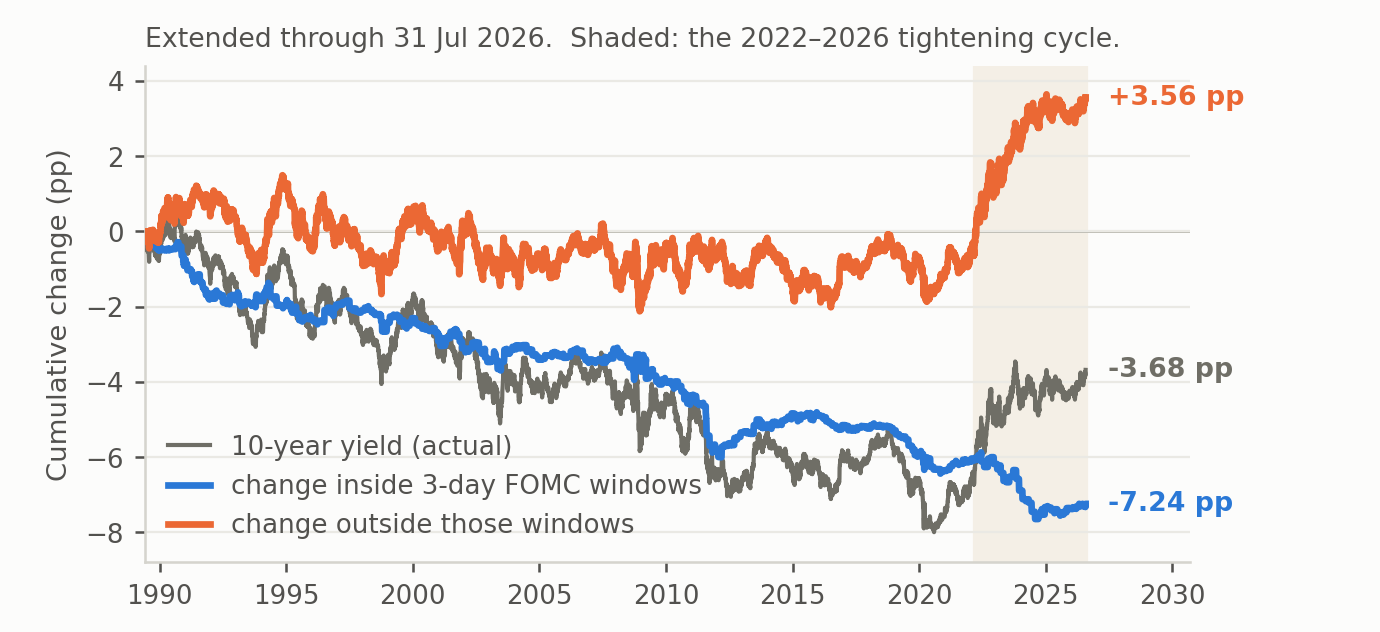
\includegraphics[width=0.78\textwidth]{s_extend.png}
\caption{\textbf{Fact 1.} Cumulative change in the ten-year yield from 2 June 1989, split into
the part accruing inside three-day FOMC windows and the part accruing on all other days.
Shaded: the 2022--2026 tightening cycle.}
\label{fig:fact}
\end{figure}
\subsection{Fact 2: the two beliefs move together, and asymmetrically}
% TODO: state the reverse-regression specification in the text (contemporaneous vs lagged
% dealer revision); the lagged version gave +0.09 (t 1.51). Regenerate 0.31/3.91 and the
% 0.60/0.58 loadings from the results file.
The FOMC publishes its longer-run funds rate projection quarterly; the NY Fed surveys primary
dealers for the same object about two weeks before every meeting. Netting the 2\% objective
from both gives two comparable measures of \rs{} (Figure~\ref{fig:beliefs}). Across 48 matched
meetings (46--47 for the revision regressions): the gap has a standard deviation of
0.105 pp and a range of $-0.11$ to $+0.30$, exceeding 25 bp at 4\% of meetings; dealers move
with the Fed nearly one-for-one ($\beta = 0.82$, $t=6.86$); the reverse relation is present but
weaker ($\beta = 0.31$, $t=3.91$).
\begin{figure}[tbp]
\centering
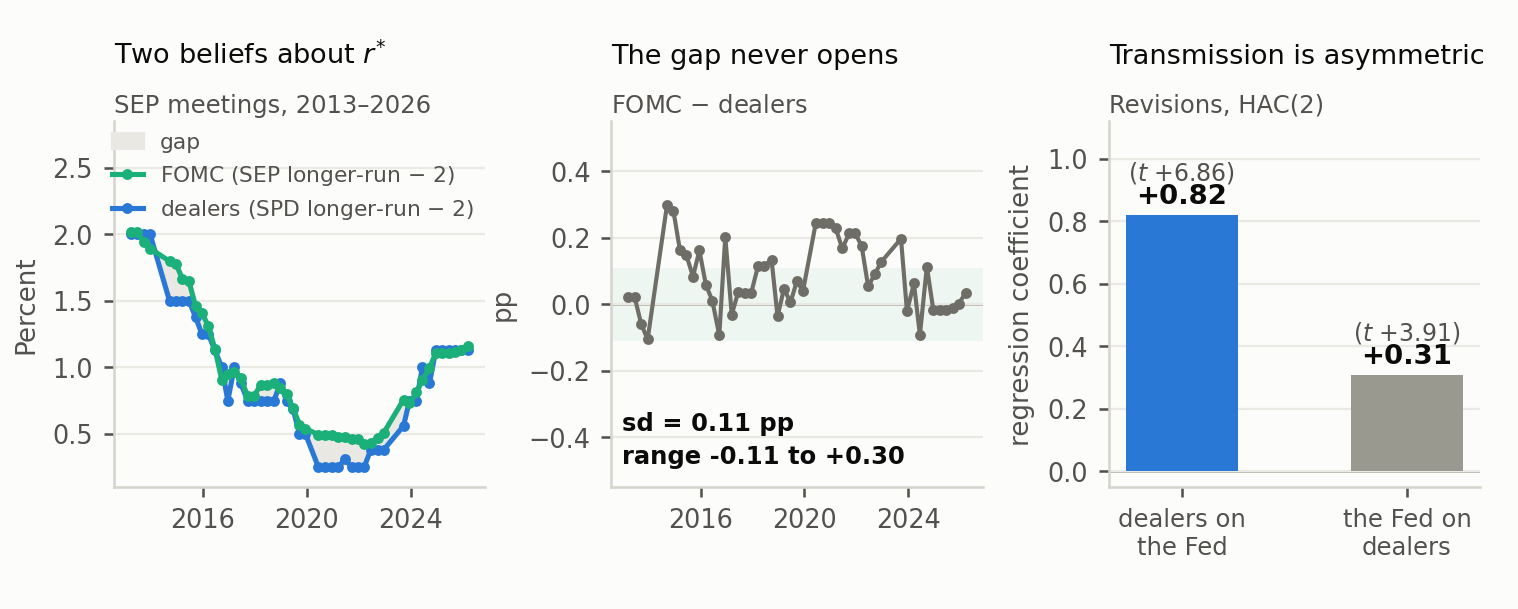
\includegraphics[width=0.82\textwidth]{s_beliefs.png}
\caption{\textbf{Fact 2.} Left: the FOMC's longer-run projection and the primary dealers'
longer-run funds rate, each less 2.0. Centre: the difference. Right: revision regressions,
HAC(2), 46--47 meetings.}
\label{fig:beliefs}
\end{figure}
The asymmetry is not mechanical --- the Desk briefs the FOMC with survey results before each
meeting --- but it is not a clean lead-lag either. Dealer revision loads on
both the preceding dot revision (0.60) and the contemporaneous one (0.58), so part of what looks
like following is anticipation; and intermeeting macro news moves both series, so these
regressions describe timing, not identified transmission. Both series are observed eight times
a year. Section~\ref{sec:tests} adds a pricing counterpart to this fact: the announcement
window prices exactly the part of the dot revision that the dealers' own preceding revision did
not anticipate.
\subsection{Fact 3: the FOMC's $r^{*}$ and the econometric $r^{*}$ move in opposite directions}
% TODO before circulating further: (1) state which HLW code/vintage produced the series;
% (2) re-run on the COVID-adjusted (2023) model; (3) check real-time vintages, which declined
% over 2012-2019; (4) report the revision-level correlation alongside -0.93.
The FOMC's estimate can be compared against the leading model-based alternative. Holston,
Laubach \& Williams estimate the equilibrium real rate from a semi-structural macro model with a
Kalman filter, quarterly from 1961. Under the martingale assumption, these two are estimates of the same object: HLW's contemporaneous
$r^{*}_t$ and the FOMC's longer-run projection coincide when $E_t[r^{*}_{t+j}] = r^{*}_t$.
They do not behave like estimates of the same object (Figure~\ref{fig:rstartwo}). Across the 57
SEP meetings the correlation of levels is $\mathbf{-0.93}$.
Between January 2012 and March 2022 the FOMC marked its own $r^{*}$ \emph{down} by 1.78 pp,
from 2.21\% to 0.42\%, while HLW marked $r^{*}$ \emph{up} by 1.37 pp, from 0.89\% to a peak of
2.26\%. After 2022 they swap: the FOMC revises up 0.74 pp while HLW falls back. The two series
cross exactly once, in June 2016, and the mean absolute gap between them is 0.88 pp --- they sit
within 25 bp of each other at only 5\% of meetings.
\begin{figure}[tbp]
\centering
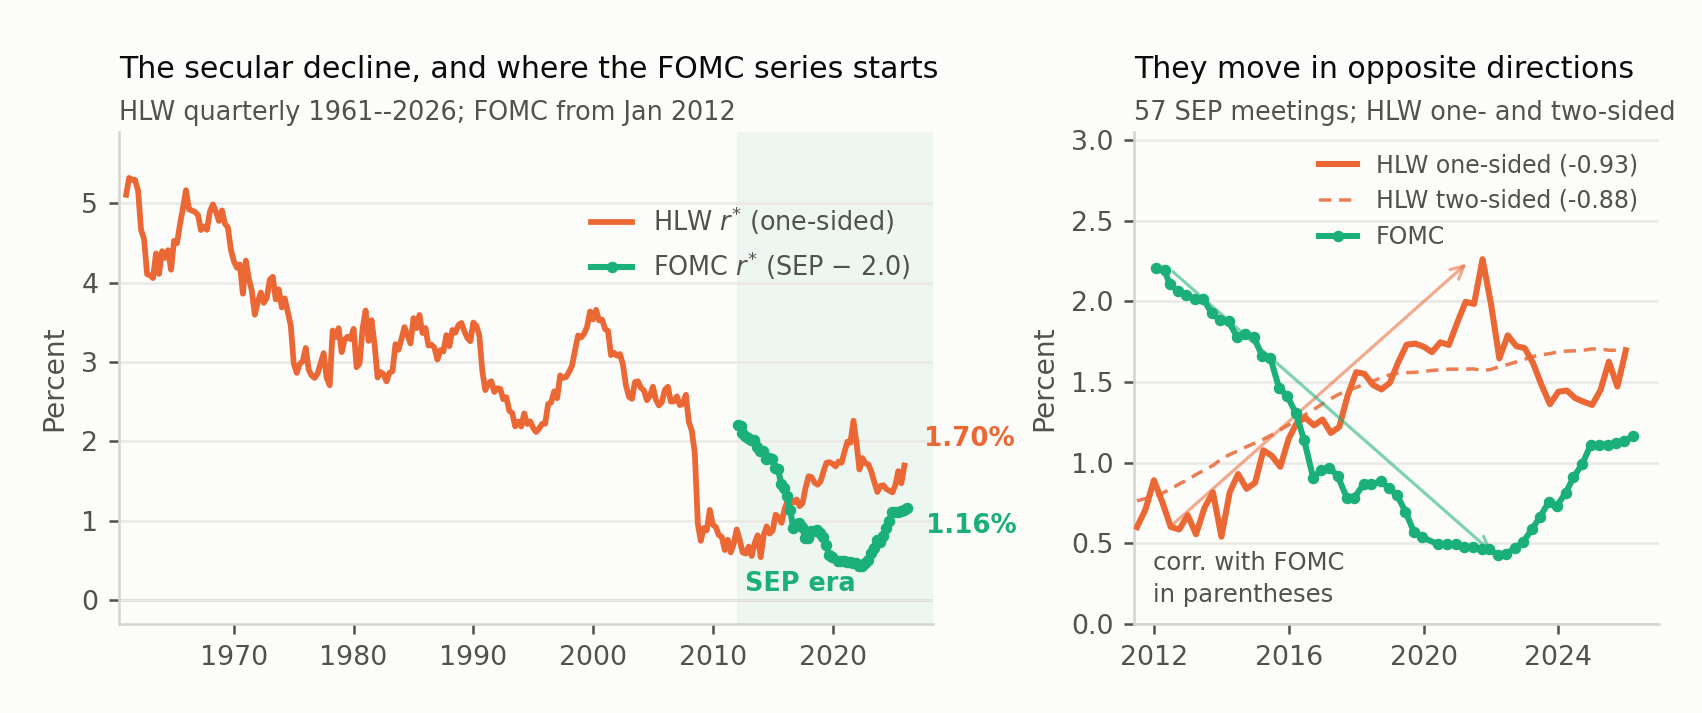
\includegraphics[width=0.95\textwidth]{s_rstar_two.png}
\caption{\textbf{Fact 3.} Left: HLW $r^{*}$ over the full quarterly sample with the FOMC series,
which begins in January 2012, overlaid; the SEP era is shaded. Right: the overlap sample, with
arrows marking the direction each series travels over 2012--2022.}
\label{fig:rstartwo}
\end{figure}
Three things follow. First, the Fed's $r^{*}$ is not easily recoverable from an econometric
model. Second, the same holds for the market side: it is hard to justify a model-based endpoint
to serve as the market perception of $r^*$. Third, the premise that the Fed holds an
information advantage about $r^{*}$ has an observable consequence: over the decade in which the
Committee cut its estimate by 1.78 pp, the filtered econometric estimate moved the other way.
The comparison uses one-sided estimates under current parameters; whether it survives on the
real-time vintages, which declined over 2012--2019, and on the post-COVID revision of the model
is being verified.
One candidate explanation can be rejected immediately. HLW estimates $r^*$ from a model; the
Fed's is inferred from its reported $i^*$ and $\pi^*$, and the SEP reports $\pi^* = 2.0\%$ with
zero variation over the observed sample. If participants report $i^*$ sincerely but hold
$\pi^*$ at 2\% to anchor expectations, the netting $r^{*}_{\text{Fed}} = \text{dot} - 2$ would
mislabel the Fed's real endpoint and the two series would not be comparable.
Figure~\ref{fig:impliedpi} tests this directly: it computes the long-run inflation expectation
that would have to be embedded in the FOMC's projection for the two estimates to agree. That
implied series runs from 3.46\% in September 2012 to 0.20\% in December 2021 --- at its trough
it requires FOMC participants to have expected 0.20\% long-run inflation at a moment when
realised inflation was 5.17\%. Whatever separates the two estimates, it is not the 2\% netting.
\begin{figure}[tbp]
\centering
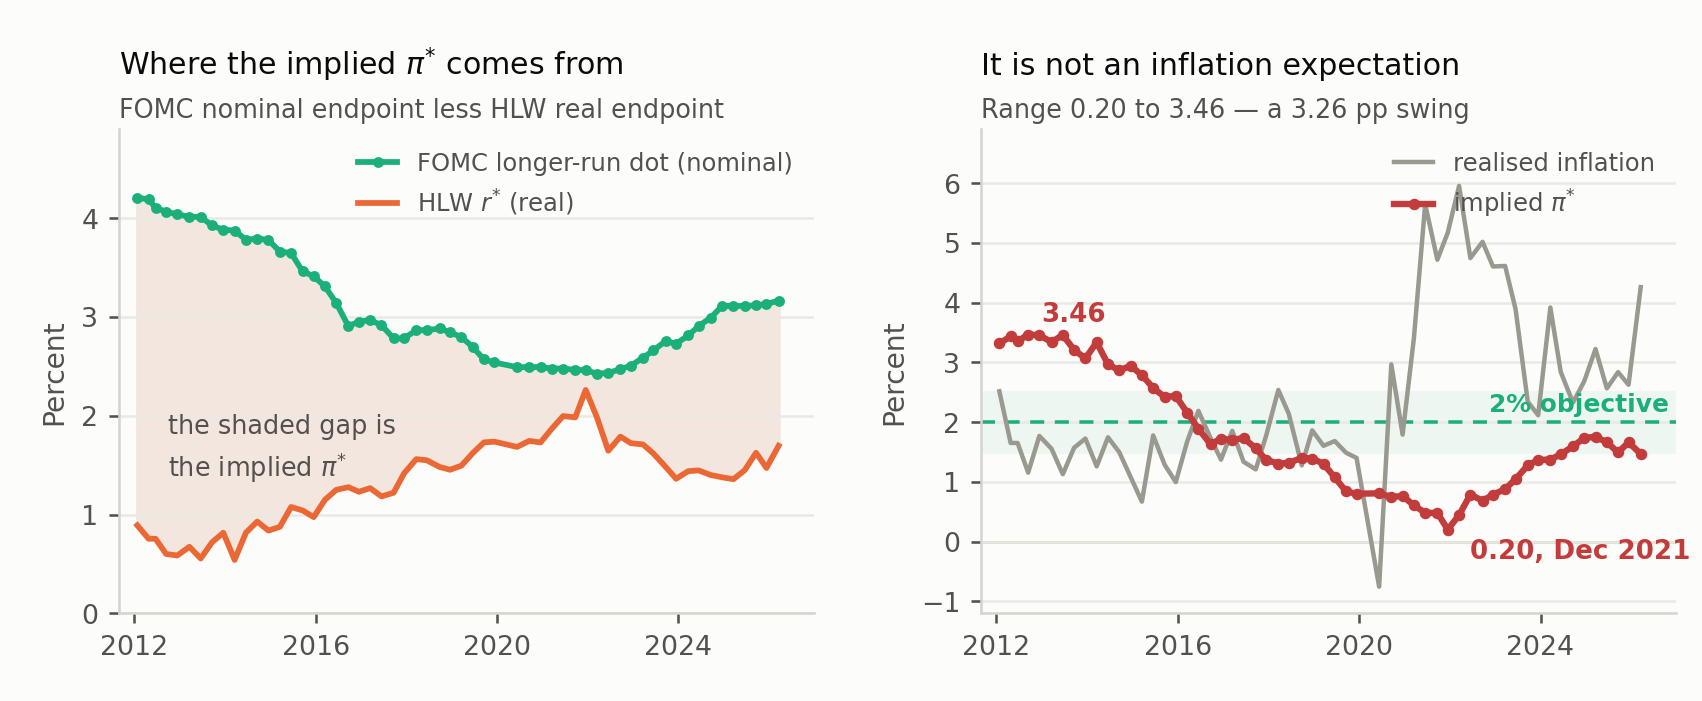
\includegraphics[width=0.95\textwidth]{s_implied_pi.png}
\caption{\textbf{The inflation expectation needed to reconcile the two estimates.} Left: the
FOMC's longer-run federal funds projection, which is nominal, against HLW's one-sided $r^{*}$,
which is real, at the 57 SEP meetings; the shaded area between them is the long-run inflation
expectation that would have to be embedded in the FOMC's projection for the two series to be
mutually consistent. Right: that implied series plotted against realised inflation, with the
2\% objective marked and a 1.5--2.5\% band shaded. The implied series lies outside the
1.5--2.5\% band at 75\% of meetings. Realised inflation is HLW's own four-quarter input series
rather than headline PCE.}
\label{fig:impliedpi}
\end{figure}
% \begin{center}\small
% \begin{tabular}{lrrr}
% \toprule
% Period & bp/meeting & $t$ & Cumulative\\ \midrule
% Jun 1989 -- Dec 2011 (pre-SEP) & $-2.46$ & $-3.06$ & $\mathbf{-5.85}$ pp\\
% Jan 2012 -- Mar 2022 (dot falling 1.78 pp) & $-0.40$ & $-0.41$ & $-0.23$ pp\\
% Mar 2022 -- Jul 2026 (dot rising 0.74 pp) & $-3.49$ & $-1.53$ & $-1.16$ pp\\
% \bottomrule\end{tabular}
% \end{center}
% \noindent 81\% of the in-window decline is complete before the dot plot begins. In the decade
% when the FOMC cut its own longer-run rate by 1.78 pp --- when an information channel should be
% loudest --- the in-window contribution is indistinguishable from zero. Every design using the
% published projection is therefore estimated on a sample in which the motivating phenomenon is
% absent. That is an argument about the whole of Component A, not one contingency within it.
% =====================================================================
\newpage
\section{Framework: intercept disagreement in an opinionated-markets model}
\label{sec:framework}
Caballero \& Simsek (2022) study a Fed and a market that disagree, each confident in its own
view, with the Fed setting policy on its belief and the market pricing assets knowing it will.
The market therefore anticipates policy ``mistakes'' and prices the resulting risk. Their state
variable is aggregate demand. This section runs the same logic with the disagreement located in
the \emph{intercept of the policy rule}. What distinguishes intercept disagreement is not its
persistence --- the estimated Fed--dealer gap mean-reverts with a half-life of about six
months --- but that it maps into a \emph{composition} restriction across the nominal and real
curves that demand disagreement does not generate.
\subsection{Setup}
Both parties know the rule and observe the state. They differ only in the neutral real rate:
the Fed believes $r^{*F}$, the market believes $r^{*m}$, and
\begin{equation}
\delta_t \;\equiv\; r^{*m}_t - r^{*F}_t .
\label{eq:delta}
\end{equation}
The Fed sets policy on its own estimate,
\begin{equation}
i_t \;=\; r^{*F}_t + \pi^{*} + \phi_\pi\!\left(\pi_t - \pi^{*}\right) + \phi_x x_t ,
\qquad \phi_\pi > 1 ,
\label{eq:rule}
\end{equation}
and the market evaluates the resulting stance against \emph{its} neutral rate, perceiving policy
to be $\delta_t$ looser than the Fed intends.
\subsection{Three roles, and whose belief enters where}
\begin{center}\small
\begin{tabular}{@{}lll@{}}
\toprule
& \textbf{Role} & \textbf{Estimate used}\\ \midrule
Fed & Sets $i_t$ through the rule \eqref{eq:rule} & $r^{*F}$\\
Economy & Adjusts $\pi$ until the real rate reaches the natural rate & the truth, $r^{*}$\\
Market & Forecasts the path of $i$; prices bonds off that forecast & $r^{*m}$\\
\bottomrule\end{tabular}
\end{center}
\noindent The market's error is that it substitutes its own $r^{*m}$ for the second row when it
runs the economy forward in its head. Long yields follow by averaging the expected short-rate
path the market computes this way; the resulting pricing equation is \eqref{eq:pricing} below.
\subsection{The market's subjective steady state}
Consider the steady state the market \emph{forecasts}, holding its belief dogmatically. Two
conditions define it. Over the long-run the Fed closes the output gap, so $\phi_x x_t$ drops
out and permanent accommodation is absorbed entirely by inflation rather than by output; and the
natural rate is by definition the real rate consistent with a zero gap, so $i-\pi$ equals the
natural rate --- which, in the market's forecast, is the one the market believes in:
$i - \pi = r^{*m}$. Substituting \eqref{eq:rule},
\[
r^{*m} \;=\; r^{*F} + \pi^{*} + \phi_\pi(\pi-\pi^{*}) - \pi
\qquad\Longrightarrow\qquad
\left(\phi_\pi-1\right)\left(\pi-\pi^{*}\right) \;=\; \delta ,
\]
so the market expects inflation to settle permanently away from target at
\begin{equation}
\boxed{\;\pi - \pi^{*} \;=\; \frac{\delta_t}{\phi_\pi - 1}\;}
\label{eq:bias}
\end{equation}
The target $\pi^{*}$ is a parameter of the
rule, set by the Fed by announcement and held at 2\% throughout the sample --- all 594 archived
longer-run PCE submissions are exactly 2.0, with zero within-meeting dispersion. What moves is
\emph{realised} long-run inflation $\pi$. The Fed does not revise its target; it persistently
misses one it continues to hold, because it is setting policy against the wrong intercept. The
adjustment runs through the real rate: at $\pi=\pi^{*}$ the real rate is $r^{*F}$, which is below
the natural rate, so demand exceeds supply and inflation rises; each point of inflation above
target raises $i$ by $\phi_\pi$ and therefore the real rate by $\phi_\pi-1$; this continues until
the real rate has climbed to meet the natural rate. Nobody chooses the natural rate, and nobody
chooses $\pi$ --- inflation is the free variable.
\paragraph{Subjective, not actual.} In the \emph{true} steady state $i-\pi = r^{*}$, and
\eqref{eq:bias} with $\delta$ replaced by $r^{*}-r^{*F}$ gives the realised bias. The market's
version coincides with it only if the market happens to be right. Nothing below requires that it
is: bonds are priced off $E^{m}_t[i_{t+j}]$, which the market computes using its own intercept at
every step, so \eqref{eq:bias} and \eqref{eq:amplification} are statements about market
expectations and hold whether or not those expectations are correct.
% This is the dogmatic-beliefs
% structure of Caballero \& Simsek, and it is the only sense in which a steady state is invoked
% here.
\paragraph{The role of the Taylor principle.} Under true dynamics the real rate is\\
$r^{*F}+(\phi_\pi-1)(\pi-\pi^{*})$, so inflation rises until the second term offsets the Fed's
intercept error, and it converges to a finite bias only because $\phi_\pi>1$.
% The same condition
% that bounds the multiplier in \eqref{eq:amplification} is what makes the steady state reachable
% at all, which is why $\phi_\pi>1$ is not an assumption of convenience.
The macro logic is Orphanides' account of the Great Inflation --- a policy rule fed a mismeasured
real-time natural rate producing a sustained inflation bias. The analogy is structural rather
than literal: Orphanides locates the mismeasurement in the output gap and the natural rate of
unemployment, i.e.\ in the $\phi_x x_t$ term, whereas the mechanism here is in the intercept.
Orphanides \& Williams on natural-rate misperception under learning is the closer antecedent.
\subsection{The amplification result, and what it does and does not identify}
The nominal endpoint the market prices is $r^{*m} + \pi^{*} + \delta/(\phi_\pi-1)$; the endpoint
the FOMC publishes is $r^{*F} + \pi^{*}$. The difference is
\begin{equation}
\boxed{\;\underbrace{i^{*m}_t - i^{*F}_t}_{\text{endpoint gap}} \;=\; \frac{\phi_\pi}{\phi_\pi-1}\;\delta_t\;}
\label{eq:amplification}
\end{equation}
\paragraph{Identification.} Given the Fed's
published $i^{*F}$, the market's expected terminal nominal rate reveals $r^{*m}$ --- but only up
to the perceived $\phi_\pi$. Equation \eqref{eq:amplification} is one equation in two unknowns:
the same observed endpoint gap is consistent with a small $\delta$ and a weakly-responding
perceived Fed, or a large $\delta$ and an aggressive one. Recovering the perceived $\phi_\pi$
from the ratio therefore requires observing $\delta$ and the endpoint gap \emph{separately},
and on current data that is not possible. The SPD's longer-run PCE median is 2.0 in every one
of the 91 surveys in the sample, so dealers condition on inflation at target and the survey gap
measures $\delta$ itself; the amplified endpoint gap does not appear in the survey. Nor can it
be taken from market prices: far-forward risk-neutral rates load heavily on the current short
rate and cannot serve as an independent endpoint. The result is therefore best read as an
identification statement: the published dot and the market's terminal rate differ by a
\emph{multiple} of the underlying disagreement, and the multiple is the perceived Taylor
coefficient. This statement does not depend on the calibration below.
\paragraph{The magnitude claim.} Read as a statement about levels, a small
disagreement about $r^{*}$ implies a large disagreement about where nominal rates would settle,
with the multiplier set by the perceived aggressiveness of the rule:
\begin{center}\small
\begin{tabular}{lccc}
\toprule
$\phi_\pi$ & inflation bias per 1 pp of $\delta$ & endpoint gap per 1 pp of $\delta$ & endpoint gap when sd$(\delta)=0.105$\\ \midrule
1.25 & 4.00 & 5.00 & 52 bp\\
1.50 & 2.00 & 3.00 & 32 bp\\
2.00 & 1.00 & 2.00 & 21 bp\\
2.50 & 0.67 & 1.67 & 18 bp\\
\bottomrule\end{tabular}
\end{center}
\noindent \textbf{These are steady-state numbers}: the multiplier is attained only if the
market expects the disagreement never to be resolved. At the estimated resolution speed --- the
Fed--dealer gap has an AR(1) coefficient of 0.849 per meeting, a half-life of about six
months --- the ten-year loading falls from its asymptotic value of 3.0 to roughly 0.1 unless
about half of any given disagreement is permanent (\S\ref{sec:path}). The table is an upper
bound, not a statement about observed magnitudes.
\paragraph{The steady state is self-defeating.} Reaching it requires the Fed to observe
inflation running $\delta/(\phi_\pi-1)$ above target --- at $\phi_\pi=1.5$, twice the size of
$\delta$ itself --- indefinitely, and never to revise $r^{*F}$. But a persistent inflation gap
is precisely the signal that identifies an intercept error. The mechanism therefore generates
the evidence that resolves the disagreement it depends on. This objection is prior to and
independent of the estimated persistence, and it is a further reason to expect the permanent
component of disagreement to be small.
\subsection{The path to the steady state}
\label{sec:path}
The steady-state gap in \eqref{eq:amplification} is the limit of a path. Along the market's
forecast, the inflation bias builds as the economy responds to the too-low real rate, and the
disagreement itself shrinks as the Fed revises $r^{*F}$ toward the market's view; a share
$\alpha$ of any given disagreement is never resolved. Parameterising the build at rate $\kappa$
and the resolution at rate $\mu$, the market's expected short rate at horizon $j$ loads on the
current disagreement as
\begin{equation}
\lambda_j \;=\; \frac{\phi_\pi}{\phi_\pi-1}\underbrace{\left(1-e^{-\kappa j}\right)}_{\text{bias builds}}
\Big[\underbrace{\alpha}_{\text{unresolved}} + \underbrace{(1-\alpha)(1-\mu)^{j}}_{\text{Fed learns}}\Big],
\qquad \alpha\in[0,1].
\label{eq:lambda}
\end{equation}
The two polar cases anchor the interpretation. At $\alpha=1$ the loading rises monotonically
with horizon and converges to the multiplier in \eqref{eq:amplification}: the amplification
result is the long-horizon limit of \eqref{eq:lambda}. At $\alpha=0$ the loading is
hump-shaped and converges to zero: under pure learning the amplified endpoint is a transient
that has largely disappeared by the maturities at which it would be priced. The two claims of
this section --- a large steady-state gap and a falsifiable hump in maturity --- therefore trade
off against each other through $\alpha$.
\paragraph{Calibration.} $\mu$ is estimated from the gap's own persistence: an AR(1)
coefficient of $0.849$ per meeting (half-life $4.2$ meetings, or $6.4$ months) gives
$\rho_{\text{month}}=0.897$ and $\hat\mu=0.103$. Setting $\kappa=0.10$ per month and
$\phi_\pi=1.5$, the averaged loading $\Lambda(n)=n^{-1}\sum_{j<n}\lambda_j$ --- which is the
coefficient a maturity regression estimates, and equals the ten-year endpoint multiplier at
$n=$ 10y --- is:
\begin{center}\small
\begin{tabular}{lccc}
\toprule
$\alpha$ & $\Lambda$, 2y & $\Lambda$, 5y & $\Lambda$, 10y\\ \midrule
0.00 & 0.47 & 0.22 & 0.11\\
0.10 & 0.60 & 0.44 & 0.37\\
0.25 & 0.80 & 0.78 & 0.77\\
0.50 & 1.14 & 1.35 & 1.42\\
1.00 & 1.81 & 2.48 & 2.74\\
\multicolumn{3}{r}{asymptote ($n\to\infty$)} & 3.00\\
\bottomrule\end{tabular}
\end{center}
\noindent At $\alpha=0$ --- pure learning at the estimated speed --- the ten-year loading is
$0.11$: a 10 bp $\delta$ moves the ten-year expectations component by about 1 bp, against 30 bp
in the steady state. Delivering even half the asymptotic multiplier requires
$\alpha\approx0.5$. Whether the amplification is quantitatively relevant therefore turns
entirely on the permanent share of disagreement, and if $\alpha$ cannot be bounded away from
zero the magnitude claim should be dropped rather than reported at its steady-state value.
\S\ref{sec:test-alpha} now bounds it from both sides: the far-forward evidence puts
$\alpha$ at about $0.25$, with a 95\% interval of roughly $[0.10,\,0.45]$, rejecting the
steady-state multiplier and pure transience alike.
\paragraph{Peak location.} With $m\equiv-\ln(1-\mu)$ and $\alpha=0$, $\lambda_j$ peaks at
\begin{equation}
j^{*} \;=\; \frac{1}{\kappa}\ln\!\left(1+\frac{\kappa}{m}\right),
\label{eq:peak}
\end{equation}
which is $6.5$ months at the calibration above. The object a maturity regression estimates is
$\Lambda$, not $\lambda$, and a running average peaks strictly later, where
$\lambda_n=\Lambda(n)$: at $12$ months for $\alpha=0$ and $28$ months for $\alpha=0.25$, moving
out and flattening as $\alpha$ rises. Both $\kappa$ and $\mu$ are estimable outside the event
sample, so the location of the peak is a quantitative prediction rather than an asserted
shape --- though the test loses power as $\alpha$ grows, since the hump flattens toward the
monotone case.
\subsection{Pricing}
Averaging the market's expected short rates gives
\begin{equation}
y^{(n)}_t \;=\; \underbrace{i^{*F}_t}_{\text{published endpoint}}
\;+\; \underbrace{\omega(\rho,n)\,\text{gap}_t}_{\text{stance}}
\;+\; \underbrace{\Lambda(n)\,\delta_t}_{\text{perceived error}}
\;+\; \underbrace{TP^{(n)}\!\left(\sigma^{2}_{\delta,t}\right)}_{\text{disagreement premium}} .
\label{eq:pricing}
\end{equation}
The yield is anchored on the Fed's \emph{published} endpoint. This is not an assumption about
whose belief is correct; it follows from the roles above. Realised short rates are generated by
the Fed's rule, so the path the market forecasts starts at the Fed's intercept, and the
market's own belief enters only through the inflation path it expects that rule to produce ---
the $\Lambda(n)\,\delta_t$ term. The two anchors are reconciled at the long end: when
$\alpha=1$, $\Lambda(n)\to\phi_\pi/(\phi_\pi-1)$ and the long yield converges to the market's
terminal rate; when $\alpha<1$, the Fed's expected learning pulls it back toward the published
endpoint. Every regressor in \eqref{eq:pricing} is observable: $i^{*F}$ is published, the
stance is measurable, and $\delta$ is the survey gap.
\subsection{Predictions}
\label{sec:predictions}
\begin{enumerate}\setlength\itemsep{0.25em}
\item \textbf{Amplification: not directly measurable on current data.} As established above,
\eqref{eq:amplification} is one equation in two unknowns, and the survey provides $\delta$ but
not the amplified endpoint gap. If an independent measure of the market's terminal rate becomes
available, the ratio identifies the market's perceived $\phi_\pi$, directly comparable to the
survey-based estimates in Bauer, Pflueger \& Sunderam (2024). Until then, the amplification
enters the empirical work only through its implications for the loadings in
\eqref{eq:pricing}.
\item \textbf{A composition restriction on the TIPS split.} The endpoint gap divides into
$\delta$ in the real dimension and $\delta/(\phi_\pi-1)$ in the inflation dimension, so
\[
\frac{\text{real endpoint gap}}{\text{breakeven gap}} \;=\; \phi_\pi - 1 .
\]
At $\phi_\pi=1.5$ breakevens move twice as much as real forwards, \emph{in the same direction}.
Demand disagreement generates no such restriction, which is what distinguishes the intercept
location. The restriction is testable on responses rather than levels: regressing far-forward
real and breakeven window changes on $\Delta\delta$ and testing that the coefficient ratio
equals $\phi_\pi-1$ requires no decomposition of either curve. The binding constraint is
power: with sd$(\delta)=0.105$ and a six-month half-life, $\Delta\delta$ has little variance,
and a power calculation must precede the test. \emph{That calculation is in
\S\ref{sec:test-power} and the test is run in \S\ref{sec:test-p2}. Two amendments follow from
it. The ratio cancels $\Lambda$, so it is free of $\alpha$ --- which makes this, not
Prediction 5, the framework's cleanest $\alpha$-free content. And it must be estimated on
$dM$ between meetings rather than on $\Delta\delta$ in the announcement window, where the
published-endpoint channel dominates.}
\item \textbf{Sign, and the absence of asymmetry.} $\delta>0$ --- the Fed's $r^{*}$ below the
market's --- means policy is perceived too easy, so both the inflation bias and the endpoint gap
are positive; $\delta<0$ reverses both. This is linearity in $\delta$, not sign-dependence:
every expression in \eqref{eq:bias}--\eqref{eq:pricing} is proportional to $\delta$, so upward
and downward disagreements are mirror images. Caballero \& Simsek's premium is genuinely
sign-dependent; this model is not, and the differentiation from them rests on the maturity
profile and the composition ratio in Prediction 2 rather than on any asymmetry. Generating
asymmetry would require a nonlinearity --- an occasionally-binding lower bound, or
state-dependent $\phi_\pi$ --- which is not in the present specification. \emph{Tested in
\S\ref{sec:test-sign}: symmetry is not rejected ($p=0.79$--$0.98$).}
\item \textbf{Maturity profile.} The three terms of \eqref{eq:pricing} carry three
distinguishable shapes: a revision to the published endpoint $i^{*F}$ loads flat, at one, across
maturity; the stance term $\omega(\rho,n)$ declines monotonically; and the disagreement term
$\Lambda(n)$ is hump-shaped for $\alpha$ small and rises monotonically toward
$\phi_\pi/(\phi_\pi-1)$ for $\alpha$ large, with the peak pinned by $(\kappa,\mu,\alpha)$ as in
\S\ref{sec:path}. \emph{Tested in \S\ref{sec:test-p4}: flat-at-one is rejected at the far
end --- the ten-year-forward pass-through of a dot revision is about one half, and
\S\ref{sec:test-p2} shows that half is entirely real.}
\item \textbf{State dependence, and a link to the perceived-slope literature.} The multiplier
$\phi_\pi/(\phi_\pi-1)$ is decreasing in $\phi_\pi$: \emph{the same $r^{*}$ disagreement matters
more when markets believe the Fed responds weakly}. Intercept disagreement and slope perception
are complements, not rival explanations --- a testable interaction, and the one prediction here
that does not depend on $\alpha$, since it concerns the shape of the multiplier in $\phi_\pi$
rather than its level. \emph{Not yet testable: it needs a perceived-$\phi_\pi$ series.
Note that Prediction 2's ratio is also $\alpha$-free, since $\Lambda$ cancels from it.}
\item \textbf{The premium.} Uncertainty about $\delta$ propagates into the whole expected path
undamped by horizon, so term-premium sensitivity to $\sigma^2_\delta$ should rise with maturity
and not decay --- unlike stance uncertainty, which is damped by $\omega$. This requires
$\sigma^2_\delta$ itself to be persistent even where $\delta$ mean-reverts; the two are separate
assumptions. The nearest existing results are Cao, Crump, Eusepi \& Moench, who show that
forecaster dispersion about the long-run level of rates accounts for roughly a third of
term-premium variation, and Cieslak, McMahon \& Pang, who show that perceived policy mistakes
move term premia rather than expected rates. The differentiation here is that the disagreement
is Fed-versus-market rather than forecaster-versus-forecaster, and is located in the intercept
of the rule, which is what generates the composition restriction in Prediction 2. \emph{A
proxy test in \S\ref{sec:test-prem} finds nothing; the proxy is weak, and the prediction
remains open.}
\end{enumerate}
\subsection{What the model assumes, stated plainly}
\emph{The permanent share $\alpha$.} The magnitude of the amplification lives or dies on it,
and the maturity-profile test loses power as it rises. In principle $\alpha$ is the unit-root
share of the Fed--dealer gap; in practice, roughly 48 observations of a series with a standard
deviation of 0.105 are unlikely to bound it tightly, so the calibration table in
\S\ref{sec:path} should be read as a sensitivity analysis rather than a set of point
predictions.
\emph{The Taylor principle.} Everything here requires $\phi_\pi>1$, and the multiplier diverges
as $\phi_\pi\to1$. That is not a defect --- the model is saying that intercept errors are
catastrophic for a weakly-responding central bank --- but it means the empirical work must bound
$\phi_\pi$ away from one, and estimates near the boundary count as evidence against the
specification rather than as very large effects.
\emph{Measurement of $\delta$.} The survey side conditions on inflation at target --- the SPD's
longer-run PCE median is 2.0 in all 91 surveys --- so the SPD gap measures $\delta$ directly.
That validates it as the regressor in Prediction 2, and it is also why the amplified endpoint
gap cannot be measured from the same source.
\emph{Linearity.} The model generates no asymmetry. The case for locating the disagreement in
the intercept rests on the composition restriction and the maturity profile, not on
sign-dependence.
% =====================================================================
\clearpage
\section{The predictions, taken to the data}
\label{sec:tests}
This section reports the first pass of the empirical program of
\S\ref{sec:predictions} on the archive behind Facts 1--3: the SEP dot-plot
panel, the SPD/SMP survey archive, the ACM daily decomposition, and the
G\"urkaynak--Sack--Wright nominal and TIPS curves, over the 48 matched meetings
of Fact 2 (2013--2026). Five of the six predictions can now be confronted with
data; Prediction 5 waits on a perceived-$\phi_\pi$ series. One result was not
predicted at all, and it is the most useful: the announcement window prices the
\emph{unanticipated component of the dot}, measured against the dealers' own
preceding revision, and prices essentially nothing else.
\subsection{Design: two revisions with different timing}
\label{sec:test-design}
Write $\delta_t = r^{*m}_t - r^{*F}_t$ from the Fact-2 panel: the Fed side is
the mean of the longer-run dots released \emph{at} meeting $t$, the market side
the SPD/SMP longer-run median from the survey fielded roughly two weeks
before. (This build reproduces Fact 2 exactly: 48 matched meetings, gap
standard deviation 0.105, revision regressions $0.82$ ($t\,6.86$) and $0.31$
($t\,3.91$).) The revision of $\delta$ between consecutive matched meetings
splits into two pieces with different information timing,
\[
\Delta\delta_t \;=\; \underbrace{dM_t}_{\substack{\text{dealer revision}\\ \text{known before the window}}}
\;-\; \underbrace{dF_t}_{\substack{\text{dot revision}\\ \text{released inside the window}}},
\]
where $dM_t$ is the change in the dealers' longer-run rate across the two
surveys and $dF_t$ the change in the mean dot across the two SEPs. The survey
closes before the three-day announcement window $[t-1,t+1]$ opens; the dot is
published inside it. Any regression of window changes on $\Delta\delta$
therefore mixes a pre-determined regressor with an announcement-day one, and
the split regression --- window change on $dM$ and $dF$ entered separately ---
is the more informative object. This turns out to matter more than power, and
it organises everything below: \emph{the announcement window identifies what
$dF$ does; the intermeeting period identifies what $dM$ does.}
Prices are taken from the ACM decomposition (total, expectations component,
term premium, maturities 1--10y) and, model-free, from GSW instantaneous
forwards --- nominal, TIPS, and inflation compensation, which satisfy
nominal $=$ real $+$ breakeven to $10^{-14}$ on the merged file, so any nominal
response splits exactly and without a decomposition step. Two practical points
matter. First, the mean of the dots is the usable Fed-side variable: it moves
at 47 of 48 meetings, where the median moves at 19 --- the earlier finding
that the survey-based wedge ``gives nothing'' was a statement about the median,
not about the object. Second, sd$(\Delta\delta)=0.117$ pp with $n=46$--$47$,
which is the arithmetic behind every power statement below.
\subsection{The power calculation Prediction 2 requires}
\label{sec:test-power}
The composition-restriction test regresses far-forward real and breakeven
window changes on $\Delta\delta$ and asks whether the coefficient ratio equals
$\phi_\pi-1$. The observed two-day window standard deviations are 10.8 bp for
the 5y5y real forward and 6.0 bp for the 5y5y breakeven; with
sd$(\Delta\delta)=0.117$ and $n=47$ this gives minimum detectable effects
(5\% size, 80\% power) of 38 bp per pp on the real leg and 21 on the breakeven
leg. Against the model's own effect sizes (the $\Lambda$ column of
\S\ref{sec:path}, divided $1{:}2$ between real and breakeven at
$\phi_\pi=1.5$): $\alpha=0$ implies real $\approx4$ and breakeven $\approx7$ bp
per pp --- invisible; $\alpha=0.25$ implies $26$ and $51$ --- the breakeven leg
detectable with simulated power $0.99$, the real leg not ($0.27$). The ratio is
the casualty: in $5{,}000$ simulated panels the median standard error of
$\hat b_{\text{real}}/\hat b_{\text{bei}}$ is $1.35$ at small effects and
reaches $0.15$ only when the real leg is $40$ bp per pp. Separating
$\phi_\pi=1.5$ (ratio $0.5$) from $\phi_\pi=2$ (ratio $1.0$) needs a ratio
standard error below about $0.25$, which requires effects an order of magnitude
above the pure-learning prediction.
The conclusion the paper anticipated is now quantitative: Prediction 2 is
feasible as a \emph{detection} test --- same-direction, breakeven-larger ---
under moderate $\alpha$, but it will not identify $\phi_\pi$ sharply at the
observed variance of $\Delta\delta$. Equation \eqref{eq:amplification}'s ``one
equation in two unknowns'' is, in practice, also one equation in too little
variance. The calculation was worth running, but it turned out not to be the
binding constraint: \S\ref{sec:test-p2} shows the timing problem of
\S\ref{sec:test-design} does more damage to the literal specification than the
standard errors do.
\subsection{A fourth fact: the window prices the dot surprise}
\label{sec:test-fact4}
The restricted regression of window changes on $\Delta\delta$ produces
coefficients that are negative, significant, and largest in the belly: the
ACM expectations component moves $-11.7$ bp per pp at 1y ($t\,{-}2.4$),
$-26.0$ at 4--5y ($t\,{-}3.8$), $-22.2$ at 10y ($t\,{-}3.8$). The sign reads
correctly once the timing is kept in mind: $\Delta\delta$ rises when dealers
revise up and the dot does not follow, and in exactly those windows yields
fall --- toward the published endpoint. Unpacking with the split regression
shows what the restricted coefficient was averaging
(Figure~\ref{fig:tests}, left):
\begin{center}\small
\begin{tabular}{ccccc}
\toprule
$n$ & $b_{dM}$ (dealer rev.) & $b_{dF}$ (dot rev.) & $b_{dM}+b_{dF}$ & $p\,(b_{dM}=-b_{dF})$\\
\midrule
2y & $-21.3$ ($t\,{-}3.5$) & $+22.0$ ($t\,{+}2.2$) & $+0.7$ (se 9.5) & 0.94\\
5y & $-26.0$ ($t\,{-}3.6$) & $+25.8$ ($t\,{+}2.7$) & $-0.2$ (se 10.0) & 0.99\\
10y & $-22.2$ ($t\,{-}3.6$) & $+23.0$ ($t\,{+}2.9$) & $+0.9$ (se 8.3) & 0.92\\
\bottomrule
\end{tabular}
\end{center}
\noindent The two coefficients are equal and opposite at every maturity ---
the equality is never rejected, $p=0.92$--$0.99$ --- so the window prices the
single variable $dF - dM$: \emph{the part of the dot revision that the
dealers' own preceding revision did not already contain}. This is the pricing
counterpart of Fact 2. There, dealer revisions load on the preceding and
contemporaneous dot revisions ($0.60$, $0.58$), so the survey is, among other
things, a forecast of the dot; here, the market's response to the announcement
is measured against precisely that forecast. It is also a discipline on
Fact 1's interpretation: the window moves attributed to $\Delta i^{*}$ are not
responses to the published revision per se, but to its innovation relative to
a measurable prior expectation --- an expectations-versus-realization
structure that the $\Delta i^{*}$ reading implicitly assumes and the split
regression now verifies. Robustness: the pattern is unchanged in the one-day
window ($-18.9/+29.8$), in both the 2013--2019 and 2020--2026 halves, and
with median dots the $dM$ side survives while the $dF$ side weakens
($+12.7$, $t\,1.5$) --- the median's 19 moves are simply too few.
\subsection{Prediction 4: the endpoint pass-through is half, and not flat}
\label{sec:test-p4}
Prediction 4 says a revision to the published endpoint loads flat, at one,
across maturity. The model-free version of the test regresses GSW
instantaneous-forward window changes on $dM$ and $dF$; the dot-revision
loading $b_{dF}(n)$ is the estimated endpoint pass-through
(Figure~\ref{fig:tests}, centre). It is $+47$ bp per pp at the 1y forward
($t\,2.8$), rises to $+74$ at 4--5y ($t\,5.2$--$5.4$), and falls to $+49$ at
the 10y forward ($t\,2.4$). Two statements follow, with different force.
The \emph{level} is rejected: at the ten-year forward the pass-through is
$0.49$ (se $0.21$), $t=-2.5$ against one. Half of a mean-dot revision
reaches the far forward curve; the model's full pass-through overstates the
long-end response by a factor of two. The \emph{shape} is suggestive but not
established: the individual contrasts $b_{dF}(4y)-b_{dF}(1y)=+27$ ($t\,1.6$)
and $b_{dF}(10y)-b_{dF}(4y)=-26$ ($t\,{-}1.3$) do not reach significance, so
a hump peaking at 4--5y is the point estimate, not a finding. Two readings
are consistent with the sub-unit level: the market treats part of a dot
revision as transitory --- the Fed-learning discount of \S\ref{sec:path}
applied to the Fed's own announcements --- or the mean dot moves at meetings
where part of the revision was already priced through other communication.
One further detail from the forwards is worth recording: beyond the 4y
forward the surprise restriction $b_{dM}=-b_{dF}$ \emph{is} rejected
($p<0.01$) --- distant forwards respond to the dot revision beyond what the
dealer revision anticipated --- while in ACM expectations space it never is.
The ACM expectations component is a filtered object with compressed
far-forward variation (the stationary-VAR critique documented in the
archive), so where the two disagree, the raw forwards carry the information.
\begin{figure}[tbp]
\centering
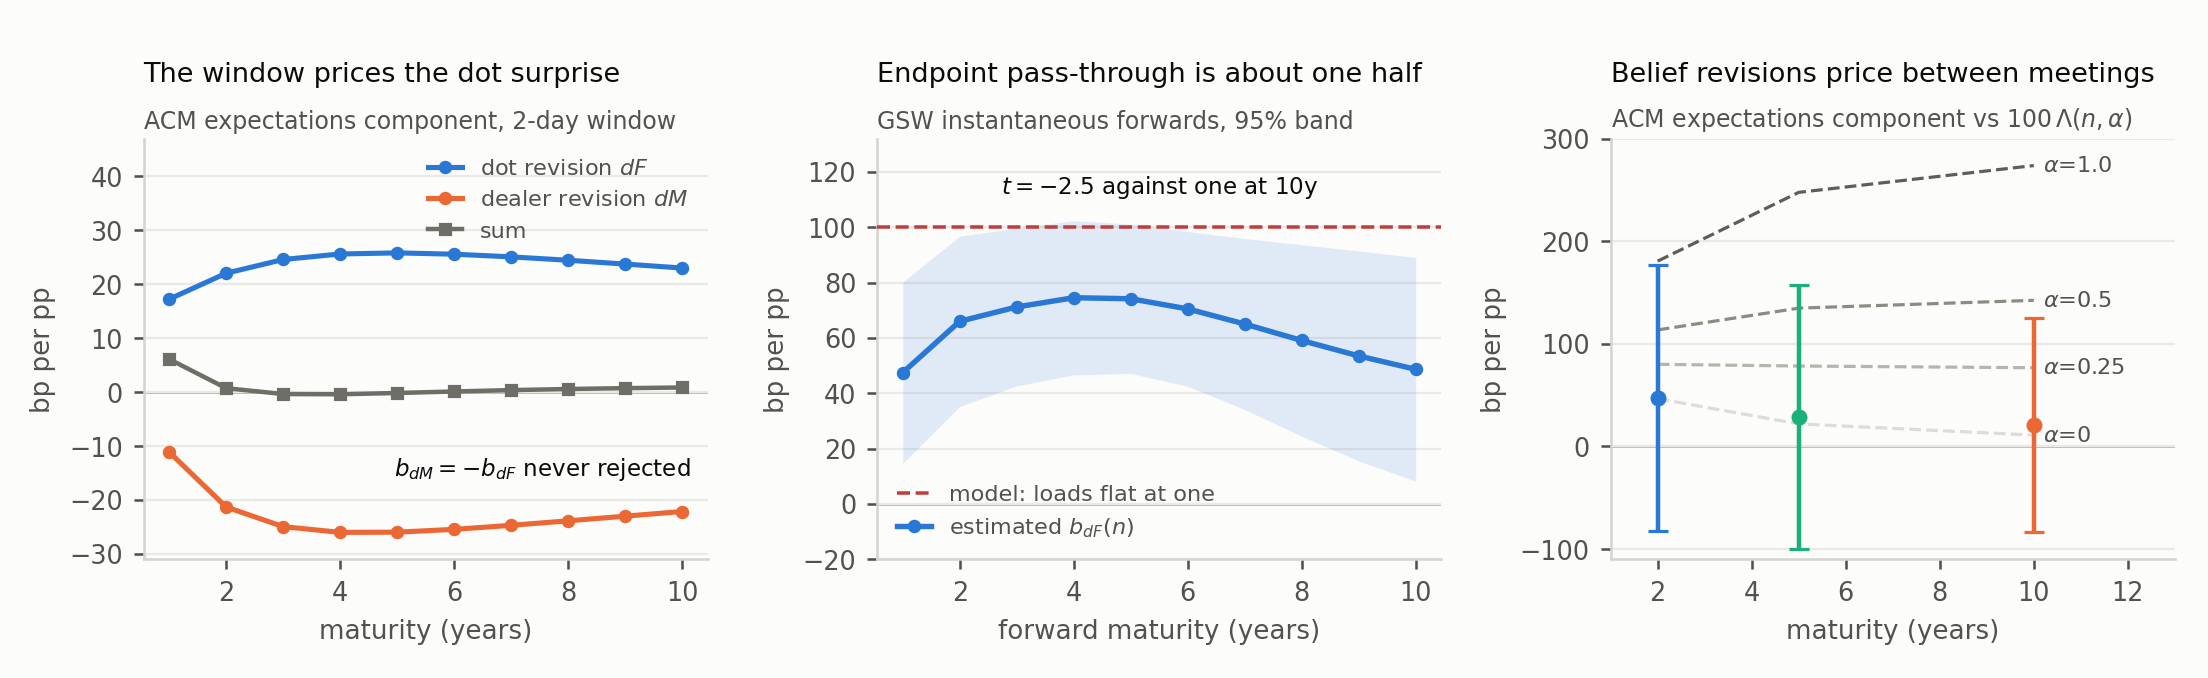
\includegraphics[width=\textwidth]{fig_tests.png}
\caption{\textbf{The dot revision and its pricing.} Left: split regression of
two-day window changes in the ACM expectations component on the dealer revision
$dM$ (pre-window) and the dot revision $dF$ (in-window), by maturity; the
coefficients are equal and opposite ($p=0.92$--$0.99$), so the window prices
the dot surprise $dF-dM$, and their sum is zero. Centre: the dot-revision
loading across GSW instantaneous forwards with 95\% bands; Prediction 4's
flat-at-one loading is drawn for reference and rejected at the far end. Right:
intermeeting pricing of dealer revisions in ACM expectations components against
the model loadings $100\,\Lambda(n,\alpha)$. HAC(4); 46--47 matched meetings,
2013--2026.}
\label{fig:tests}
\end{figure}
\subsection{Prediction 2: the composition restriction}
\label{sec:test-p2}
The TIPS curve makes the composition test operational. Its attraction is that
the ratio is \emph{free of} $\alpha$: the real and breakeven loadings are
$\Lambda(n)(\phi_\pi-1)/\phi_\pi$ and $\Lambda(n)/\phi_\pi$, so the common
$\Lambda$ cancels and the ratio is $\phi_\pi-1$ whatever the permanent share.
This makes Prediction 2, not Prediction 5, the cleanest $\alpha$-free content
of the framework. But the ratio is a ratio \emph{of responses to a movement in
$\delta$}, and by \S\ref{sec:test-design} the announcement window does not
deliver one: a dot revision moves the published endpoint and $\delta$ at the
same instant. Three specifications separate the cases.
\paragraph{(A) The composition of a dot revision.} Regress window changes on
$dF$. Since $\pi^{*}$ is 2.0 in every SEP, a dot revision \emph{is} a real
endpoint revision, and the model predicts it arrives almost entirely in the
real leg, with a small negative breakeven response from the induced fall in
$\delta$: $b_{\text{real}} = 1 - (1-\theta)\lambda(\phi_\pi-1)/\phi_\pi$ and
$b_{\text{bei}} = -(1-\theta)\lambda/\phi_\pi$, where $\theta$ is the share of
the revision the market adopts into its own belief inside the window. The data
(Figure~\ref{fig:tips}, left) are emphatic:
\begin{center}\small
\begin{tabular}{cccc}
\toprule
forward & real (TIPS) & breakeven & nominal\\
\midrule
2y & $+42.4$ ($t\,2.32$) & $-11.9$ ($t\,{-}1.40$) & $+30.5$ ($t\,2.23$)\\
5y & $+53.8$ ($t\,3.90$) & $+1.2$ ($t\,0.17$) & $+55.0$ ($t\,4.47$)\\
10y & $+44.7$ ($t\,4.82$) & $-0.1$ ($t\,{-}0.01$) & $+44.6$ ($t\,3.91$)\\
5y5y & $+51.7$ ($t\,5.03$) & $+0.9$ ($t\,0.10$) & $+52.3$ ($t\,4.97$)\\
\bottomrule
\end{tabular}
\end{center}
\noindent \textbf{The half pass-through of \S\ref{sec:test-p4} is entirely
real.} Breakevens do not move on a dot revision at any forward maturity beyond
three years; the largest breakeven coefficient anywhere on the curve is
$-11.9$ bp per pp at the 2y forward, $t\,{-}1.40$. This is Hillenbrand's
composition result --- the decline is in TIPS, not breakevens --- reproduced at
the meeting frequency and on the published projection specifically, and it is
the sharpest available evidence that the market reads the SEP longer-run dot as
a statement about the real endpoint rather than about the inflation anchor.
That is the interpretation \eqref{eq:pricing} requires, and it had not been
tested directly.
\paragraph{(B) The composition of a disagreement.} The ratio test needs a
movement in $\delta$ that does not touch the published endpoint, which is what
$dM$ is. Regressing the intermeeting change --- the close two days before
meeting $t$ against the close after meeting $t-1$ --- on $dM$
(Figure~\ref{fig:tips}, centre):
\begin{center}\small
\begin{tabular}{cccccc}
\toprule
forward & real & breakeven & ratio & Fieller 95\% (ratio) & implied $\phi_\pi$\\
\midrule
9y & $+99.1$ ($t\,2.24$) & $+52.9$ ($t\,2.44$) & $1.87$ & $[0.66,\,3.52]$ & $[1.66,\,4.52]$\\
10y & $+95.6$ ($t\,2.16$) & $+55.1$ ($t\,3.02$) & $1.74$ & $[0.33,\,2.86]$ & $[1.33,\,3.86]$\\
\bottomrule
\end{tabular}
\end{center}
\noindent Three things to take from this, in descending order of confidence.
First, \textbf{the two legs move together}, which is the model's qualitative
requirement and the feature that demand disagreement does not generate; the
contaminated specifications in (A) and (C) both show opposite signs, so this is
not an artefact of the data always co-moving. Second, the point estimate,
$\phi_\pi\approx2.7$, is higher than the $1.5$ used for calibration, and its
interval comfortably contains $1.5$; it should be read as a first estimate
rather than a number to build on. Third, and most tentatively, the ratio is
probably positive, which would put $\phi_\pi$ above one --- the check
\S\ref{sec:framework} demands of the empirical work. The evidence for that is
weaker than the Fieller intervals suggest: resampling the panel directly gives
$\Pr(\text{ratio}>0)=0.97$ (iid) and $0.95$ (moving block, $L=6$), with
percentile intervals of $[-0.17,\,4.11]$ and $[-0.78,\,4.00]$ that include
zero. The Taylor principle is favoured by the data at roughly one-sided 95\%,
not confirmed at conventional two-sided levels. Intervals are Fieller rather than delta-method
because the denominator is imprecise --- at every forward maturity except 9 and
10 years the 95\% set is unbounded, which is exactly the failure mode
\S\ref{sec:test-power} predicted, and a reason not to lean on the two
maturities where it happens to close.
The caveat is the design, not the arithmetic. An intermeeting window is six to
eight weeks of macro news, and dealers revise $r^{*m}$ in response to the same
news that moves real rates and inflation compensation directly; this is a
correlation with the right sign and the right ordering, not an identified
response. Conditioning on the intermeeting move in the 2y and 3y nominal
forwards --- the nearest available proxy for the common cycle --- leaves the
ratio at $1.81$ but widens the interval to include zero, and dropping 2020
leaves $1.83$ with an interval of $[-0.08,\,3.22]$. The composition
restriction is therefore \emph{consistent with} the data and now has a first
estimate; it is not yet established.
\paragraph{(C) The literal specification.} Regressing window changes on
$\Delta\delta$, as \S\ref{sec:predictions} originally proposed, gives
$-14.1$ ($t\,{-}0.96$) real and $+4.8$ ($t\,0.51$) breakeven at the 10y
forward, and $-65.4$ ($t\,{-}3.24$) and $+19.0$ ($t\,1.61$) at 2y: opposite
signs, which the model forbids, and a ratio near $-3$. This is not evidence
against the model. It is the timing problem: the window regression on
$\Delta\delta$ is dominated by $dF$, whose composition is the near-pure real
response of (A), so the specification measures the composition of an endpoint
revision and reports it as though it were the composition of a disagreement.
The lesson for the draft is that Prediction 2 must be stated on $dM$ and
estimated between meetings, not on $\Delta\delta$ in the window.
\begin{figure}[tbp]
\centering
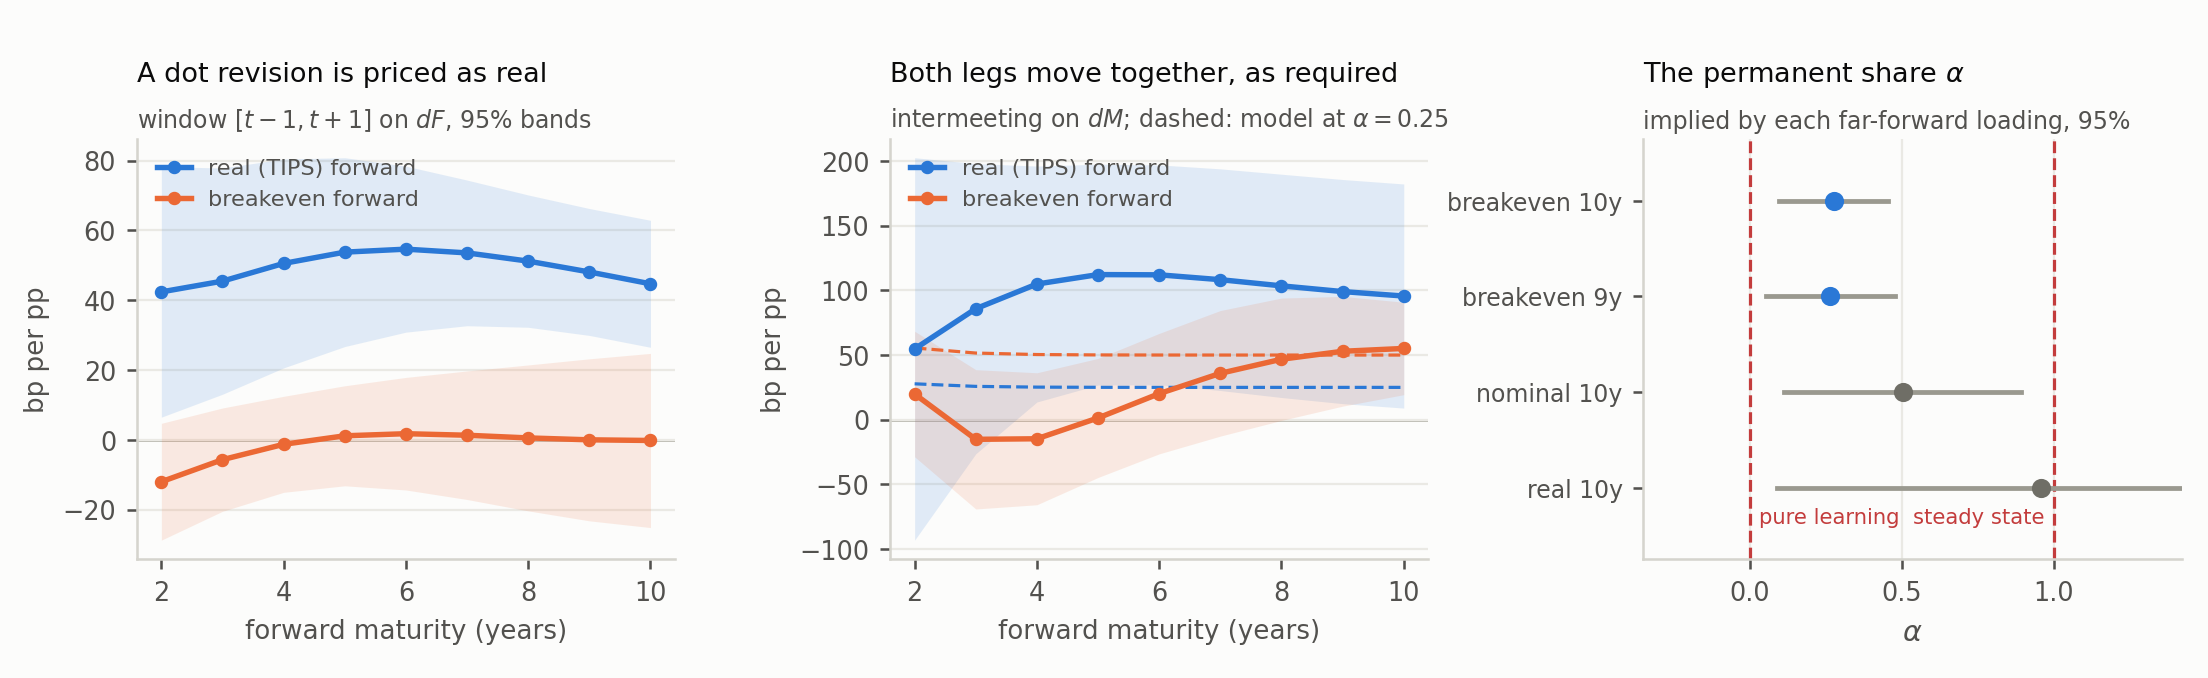
\includegraphics[width=\textwidth]{fig_tips.png}
\caption{\textbf{The composition restriction.} Left: window changes in GSW real
(TIPS) and breakeven instantaneous forwards regressed on the dot revision
$dF$ --- the response is entirely real at every maturity beyond three years.
Centre: the same two legs regressed on the dealer revision $dM$ between
meetings, with the model's predicted loadings at $\alpha=0.25$ dashed; both
legs move together, as the model requires and as the window specifications do
not. Right: the permanent share $\alpha$ implied by each far-forward loading,
where $\lambda_{120}\to3\alpha$ makes the ten-year instantaneous forward a
near-pure reading of $\alpha$; $\alpha=0$ and $\alpha=1$ are marked. HAC(4),
95\% intervals; Fieller intervals for ratios.}
\label{fig:tips}
\end{figure}
\subsection{Bounding the permanent share $\alpha$}
\label{sec:test-alpha}
The amplification term $\Lambda(n)\,\delta_t$ is the model's channel from
disagreement to the level of yields, and \S\ref{sec:path} showed its magnitude
turns entirely on $\alpha$. The far-forward data bound it from both sides.
The instrument is \eqref{eq:lambda} evaluated at a long horizon rather than
averaged. An instantaneous forward $j$ months ahead loads $\lambda_j$, and at
$j=120$ the transient factor $(1-\mu)^{j} = 0.897^{120} = 2\times10^{-6}$ is
dead, so
\[
\lambda_{120} \;\to\; \frac{\phi_\pi}{\phi_\pi-1}\,\alpha \;=\; 3\alpha ,
\]
and the real and breakeven legs load $100\alpha$ and $200\alpha$ bp per pp.
\emph{The ten-year instantaneous forward is a near-pure reading of the
permanent share}, and the breakeven leg is the best-measured of the three,
and the only one whose interval is stable under resampling (moving-block
bootstrap median $0.25$, 95\% $[0.05,\,0.45]$, $\Pr(\alpha>0)=0.99$).
From the intermeeting regressions of (B):
\begin{center}\small
\begin{tabular}{lccc}
\toprule
& coefficient & implied $\alpha$ & 95\% interval\\
\midrule
10y forward, breakeven & $+55.1$ (se 18.2) & $\mathbf{0.28}$ & $[0.10,\,0.45]$\\
9y forward, breakeven & $+52.9$ (se 21.7) & $0.26$ & $[0.05,\,0.48]$\\
10y forward, nominal & $+150.8$ (se 59.8) & $0.50$ & $[0.11,\,0.89]$\\
10y forward, real & $+95.6$ (se 44.2) & $0.96$ & $[0.09,\,1.82]$\\
\bottomrule
\end{tabular}
\end{center}
\noindent The breakeven reading survives the same robustness that weakened the
ratio: $\alpha=0.25$, $[0.06,\,0.43]$ excluding 2020, and $\alpha=0.19$,
$[0.02,\,0.37]$ conditioning on the 2y and 3y nominal forward moves. So a
one-sentence summary of the amplification mechanism is now available:
\emph{$\alpha$ is about a quarter, and both polar cases are rejected}. The
steady-state case $\alpha=1$ --- the multiplier of \eqref{eq:amplification}
taken at face value --- is excluded by every column. Pure learning,
$\alpha=0$, is excluded by the breakeven columns, which is the more interesting
of the two rejections: the calibration of \S\ref{sec:path} treated
$\alpha\approx0$ as the case that would kill the magnitude claim, and it does
not hold. At $\alpha=0.25$ the ten-year endpoint multiplier is
$\Lambda=0.77$: a 10 bp disagreement moves the ten-year expectations component
about 8 bp, against 1 bp under pure learning and 27 bp in the steady state.
Two consistency checks. The announcement-window evidence gives the same upper
bound from an independent direction. In the window, dealer belief revisions are
pre-determined, and the sum $b_{dM}+b_{dF}$ of \S\ref{sec:test-fact4} would
capture $\Lambda$ only if beliefs reached prices solely at announcements; it is
zero everywhere ($+0.9$ bp per pp at 10y, se $8.3$, block-bootstrap 95\% CI
$[-14.9,\,+17.8]$), which is what continuous pricing predicts and therefore
tells us nothing about $\alpha$ by itself. The window breakeven response to
$dF$ is more informative, but only conditionally: it bounds
$(1-\theta)\alpha$, where $\theta$ is in-window belief adoption. At
$\theta=0$ it gives $\alpha\le0.13$; at $\theta=0.5$, $\alpha\le0.25$; at
$\theta=0.82$ --- the Fact-2 survey-to-survey adoption coefficient, the most
generous case --- $\alpha\le0.70$. Since $\theta$ is unobserved, this is a
range that brackets the intermeeting estimate rather than an independent test,
but it does not contradict it. And the ACM expectations components at the yield
level, regressed on $dM$ intermeeting, give $\alpha\le0.43$ at ten years
(Figure~\ref{fig:tests}, right) --- an upper bound from a filtered, model-based
measure that lands within 0.02 of the raw-forward interval's upper end.
Three measurements, two of them independent, agree on the ceiling.
For the draft this resolves the instruction of \S\ref{sec:path} in the least
drastic direction available: the magnitude claim need not be dropped, but it
must be restated at $\alpha\approx0.25$ rather than at the steady state, where
it is roughly a quarter of the headline multiplier and still economically
meaningful. The peak-location test \eqref{eq:peak} remains unrun --- it
presupposes a $\Lambda$ profile precise enough to locate a maximum, and the
intermeeting standard errors do not support one. The hump that \emph{is} in the
data (\S\ref{sec:test-p4}) belongs to the dot-surprise loading, a different
object, with a peak at 4--5y rather than the 1--2.5y the $\Lambda$ family
predicts.
\subsection{Prediction 3: symmetry survives}
\label{sec:test-sign}
Splitting the level response at $\delta=0$ (10y, two-day window):
$p$(symmetric) $=0.98$ for the total yield, $0.79$ for the expectations
component, $0.87$ for the term premium. The model's linearity --- the
feature that distinguishes it from Caballero \& Simsek's sign-dependent
premium --- is not rejected, and the earlier appearance of asymmetry in the
ACM-based wedge does not reappear in the survey-based measure, consistent
with its being the regime artefact the gate analysis suspected. One flag for
completeness: in revisions, the ten-year term-premium response is asymmetric
(extra slope for $\Delta\delta>0$ of $-65$, $t\,{-}2.1$, $p=0.035$) --- one
rejection among ten symmetry tests, on 46 observations, worth re-checking
when the sample grows rather than interpreting now.
\subsection{Prediction 6: nothing on the available proxy}
\label{sec:test-prem}
The disagreement premium requires $\sigma^2_{\delta,t}$, which no survey
measures. The nearest available object is the dealers' cross-sectional IQR
of the longer-run rate (91 surveys, mean $0.45$, AR(1) $0.58$). ACM term
premia show no sensitivity to it at any maturity --- levels flat with
$|t|<0.9$ everywhere, changes negative and insignificant, and no rise with
maturity, which is the signature the prediction needs. The caveat cuts both
ways: forecaster dispersion is dispersion \emph{within} the market, not
uncertainty about the Fed--market gap, so this is a test of a proxy, not of
the prediction. But it removes the easy version of the result: whatever Cao,
Crump, Eusepi \& Moench's dispersion factor is picking up in term premia, the
dealers' longer-run IQR alone does not reproduce it on this sample.
\subsection{Where this leaves the program}
The empirical section of the paper changes in five ways. Fact 2 gains its
pricing counterpart --- the fourth fact of \S\ref{sec:test-fact4} --- which is
also the cleanest evidence yet for the anchoring claim of \eqref{eq:pricing}:
yields are organised around the Fed's published endpoint, to the point that the
announcement response is a pure surprise response with the dealers' survey as
the measurable expectation. Prediction 4 acquires a number: the far-forward
pass-through of a dot revision is one half, not one, and \S\ref{sec:test-p2}
shows that half is entirely real --- which both confirms the framework's
reading of the SEP dot as a real-endpoint statement and reproduces
Hillenbrand's TIPS-versus-breakevens composition on the published projection
itself. Prediction 2 becomes operational, with the caveat that it must be
estimated between meetings rather than in the window; it delivers the model's
qualitative requirement (both legs, same sign), a first ratio estimate implying
$\phi_\pi\approx2.7$, weak one-sided support for $\phi_\pi>1$, and a clear
statement of what would sharpen it. The amplification mechanism is
disciplined to $\alpha\approx0.25$ with a 95\% interval of roughly
$[0.10,\,0.45]$, so both the steady-state multiplier and pure transience are
rejected and the ten-year endpoint loading is about $0.8$. And Prediction 6
remains genuinely open, awaiting a credible measure of $\sigma^2_\delta$ rather
than a dispersion proxy.
Two vulnerabilities are worth stating in the same breath as the results. The
intermeeting design that carries Prediction 2 and the $\alpha$ bound cannot
separate the model's mechanism from common macro news; an instrument for
dealer belief revisions, or a higher-frequency survey, is the natural next
step. And the sample is what it is: sd$(\Delta\delta)=0.117$ on 46 meetings,
so everything here is a statement about small revisions to a small gap, and
the program's power grows only at eight observations a year.
\vspace{0.9em}
\noindent\rule{\textwidth}{0.4pt}\\[0.2em]
\scriptsize\textbf{Key references.} Bauer, Pflueger \& Sunderam (2024), \emph{QJE}. Bauer \&
Rudebusch (2020), \emph{AER}. Caballero \& Simsek (2022), \emph{AER}. Cao, Crump, Eusepi \&
Moench, FRBNY SR 934. Cho \& Williams (2026), Liberty Street Economics. Cieslak, McMahon \&
Pang, SSRN 4920858. Engstrom, FEDS 2026-026. G\"urkaynak, Sack \& Swanson (2005). G\"urkaynak,
Sack \& Wright (2007; 2010), \emph{JME}; \emph{AEJ:Macro}. Hanson,
Lucca \& Wright (2021), \emph{QJE}. Hartley (2025), Mercatus WP. Hillenbrand (2025),
\emph{RFS}. Holston, Laubach \& Williams (2017), \emph{JIE}; (2023), FRBNY SR 1063. Joslin,
Singleton \& Zhu (2011), \emph{RFS}. Kozicki \& Tinsley (2001), \emph{JME}. Lou, Pint\'er,
\"Usl\"u \& Walker, BIS WP 1232. Lucca \& Moench (2015), \emph{JF}. Orphanides (2003),
\emph{JME}. Orphanides \& Williams (2002), \emph{BPEA}. Pan \& Peng, SSRN 4764451. Swanson
(2021), \emph{JME}.
\end{document}
